%%%%%%%%%%%%%%%%%%%%%%%%%%%%%%%%%%%%%%%%%%%%%%%%%%%%%%%%%%%%%%%%%%%%%%%%%%%
%
%    phase1-AR.tex  (use only for Archival Research and Theory proposals; use phase1-GO.tex
%                     for General Observer and Snapshot proposals and phase1-DD.tex for GO/DD 
%                     proposals or use phase1-MC.tex for GO/MC rapid response proposals.
%                     
%
%    HUBBLE SPACE TELESCOPE
%    PHASE I ARCHIVAL & THEORETICAL RESEARCH PROPOSAL TEMPLATE 
%    FOR CYCLE 25 (2017)
%
%    Version 1.0, January 2017
%
%    Guidelines and assistance
%    =========================
%     Cycle 25 Announcement Web Page:
%
%         http://www.stsci.edu/hst/proposing/docs/cycle25announce 
%
%    Please contact the STScI Help Desk if you need assistance with any
%    aspect of proposing for and using HST. Either send e-mail to
%    help@stsci.edu, or call 1-800-544-8125; from outside the United
%    States, call [1] 410-338-1082.
%
%%%%%%%%%%%%%%%%%%%%%%%%%%%%%%%%%%%%%%%%%%%%%%%%%%%%%%%%%%%%%%%%%%%%%%%%%%%

% The template begins here. Please do not modify the font size from 12 point.

\documentclass[12pt]{article}


%%%%%%%%%%%%%%%%%%%%%%%%%%%%%%%%%%%%%%%%%%%%%%%%%%%%%%%%%%%%%
%  PREAMBLE: sets up compiler modes, loads packages, defines macros, etc
%  Steve Rodney, 2012
%%%%%%%%%%%%%%%%%%%%%%%%%%%%%%%%%%%%%%%%%%%%%%%%%%%%%%%%%%%%%


%%%%%%%%%%%%%%%%%%%%
% COMPILER MODES
%%%%%%%%%%%%%%%%%%%%

% Changetext mode : highlight modified text in bold blue font
\newif{\ifchangetext}
\changetextfalse

%% Read in the -options.tex file (generated by the Makefile)
%%  to set the compile-mode options
\InputIfFileExists{\jobname-options}


%%%%%%%%%%%%%%%%%%%%%%%%%%%%%%%
% changetext  mode settings
%%%%%%%%%%%%%%%%%%%%%%%%%%%%%%%
\ifchangetext
  % Changed text is highlighted in bold, blue font 
  \newcommand{\change}[1]{\textcolor{blue}{ \bf #1}}
  \newcommand{\changenote}[1]{\textcolor{blue}{ \bf #1}}
\else
  % Changed text is indistinguishable
  \newcommand{\change}[1]{#1}
  \newcommand{\changenote}[1]{}
\fi


%%%%%%%%%%%%%%%%%%%%
% PACKAGES INCLUDED
%%%%%%%%%%%%%%%%%%%%
%\usepackage{deluxetable}  % stand-alone version of AAStex's  deluxetable
\usepackage{longtable}
\usepackage{tabu}
\usepackage{booktabs}
\usepackage{array}
\usepackage{aas-macros}
\usepackage{phase1}
\usepackage{url}
%\usepackage{journalnames} % Astro Journal abbreviations
\usepackage{natbib}   % reference citations and bibliography
\usepackage[svgnames]{xcolor}  % colored text (better than color)
\usepackage{graphicx}
\usepackage{amsmath}  % equations and such
%\usepackage{amssymb}  % extended symbols lib
\usepackage{setspace} % switch from double to single spacing
\usepackage{wrapfig}
\usepackage{float}
\usepackage[font=small]{caption}
\usepackage{subcaption}
\usepackage{hyperref}

%\usepackage[linkcolor=blue,citecolor=darkgray,colorlinks=true]{hyperref}
%\usepackage{enumerate}% enumerated lists
%\usepackage{mathrsfs} % extended math fonts (mathscr)
%\usepackage{breqn}    % automatic line breaks for long equations
%\usepackage{multirow}  % muti-row table cells
%\usepackage{paralist} % inline enumeration (for Table ref lists)
%\usepackage{authblk}
%\usepackage{multicol}
\usepackage{sidecap} % captions beside figs
%\usepackage{subfig} % subfloats with independent captions
%\usepackage{subcaption} % subfloats with independent captions
%\usepackage[none]{hyphenat} % Suppress the hyphenating
%\usepackage{verbatim} % verbatim text formatting
%\usepackage{ulem} % for some underlining.
%\usepackage[usenames]{color}  % colored text
%\usepackage{colortbl}


\usepackage{multicol}

%\usepackage{etoolbox}
%\patchcmd{\thebibliography}{\section*{\refname}}
%    {\begin{multicols}{2}[\section*{\refname}]}{}{}
%\patchcmd{\endthebibliography}{\endlist}{\endlist\end{multicols}}{}{}

%%%%%%%%%%%%%%%%%%%%%%%%%%%%%%%%%%%%%%%%%%%%%%%%%%%
% PDF mode settings : Auto-select eps or pdf figures 
% based  on the compiler used (i.e. latex vs pdflatex)
%%%%%%%%%%%%%%%%%%%%%%%%%%%%%%%%%%%%%%%%%%%%%%%%%%%
%\DeclareGraphicsExtensions{.png,.pdf,.jpg}

%%%%%%%%%%%%%%%%%%%%%%%%%%%%%%%
% AUTHOR-DEFINED MACROS
%%%%%%%%%%%%%%%%%%%%%%%%%%%%%%%

% Time delay 
\def\dt{\ensuremath{\Delta t}}
\def\Dl{\ensuremath{D_L}}
\def\Ds{\ensuremath{D_S}}
\def\Dls{\ensuremath{D_{LS}}}

% dagger for marking primary targets
\def\dag{\ensuremath{^{\dagger}}}

% plus-minus symbols for statistical or systematic errors
\def\pmstat{\ensuremath{\substack{\pm \\ \mbox{\scalebox{0.45}{stat}}}}}
\def\pmsys{\ensuremath{\substack{\pm \\ \mbox{\scalebox{0.45}{sys}}}}}


% prompt Ia fraction
\def\fp{\ensuremath{f_{P}}}
\def\fP{\ensuremath{f_{P}}}

% STARDUST probabilities
\def\pIa{\ensuremath{p_{Ia}}}
\def\pIaz{\ensuremath{p_{Ia,z}}}
\def\pIahost{\ensuremath{p_{Ia,host}}}

% General purpose usefulness:
\newcommand{\etal}{{et al.~}}                                             
\def\eg{{e.g.}}
\def\ie{{i.e.}}
\def\etc{{etc.}}
\newcommand{\lta}{\lesssim}                                               
\newcommand{\gta}{\gtrsim}                                                
\newcommand{\gt}{\gtsim}

% Cosmology:
\def\Om{\ensuremath{\Omega_{\rm m}}}
\def\Ot{\ensuremath{\Omega_{\rm tot}}}
\def\Ob{\ensuremath{\Omega_{\rm b}}}
\def\OL{\ensuremath{\Omega_{\Lambda}}}
\def\Ok{\ensuremath{\Omega_{\rm k}}}
\def\om{\ensuremath{\omega_{\rm m}}}
\def\ob{\ensuremath{\omega_{\rm b}}}
\def\wo{\ensuremath{w_0}}
\def\wa{\ensuremath{w_{\rm a}}}
\def\lcdm{$\Lambda$CDM}
\def\LCDM{$\Lambda$CDM}
\def\wcdm{$w$CDM}
\def\Ho{\ensuremath{H_0}}
\def\DA{\ensuremath{D_A}}
\def\DL{\ensuremath{D_L}}

% Astronomy:
\def\arcsec{\ensuremath{^{\prime\prime}}} 
\def\kms{\ensuremath{{\rm km s}^{-1}}}
\def\hgpcq{\mbox{$h^{-3}$Gpc$^3$}}
\def\hmpcq{\mbox{$h^{-3}$Mpc$^3$}}
\def\perhmpcq{\mbox{$h^{3}$Mpc$^{-3}$}}
\def\hmpc{\mbox{$h^{-1}$Mpc}}
\def\hmpci{\mbox{$h$\,Mpc$^{-1}$}}
\def\mpc{\mbox{Mpc}}
\def\mpci{\mbox{Mpc$^{-1}$}}
\def\mpcq{\mbox{Mpc$^{-3}$}}
\def\Msun{\mbox{M$_{\odot}$}}
\def\Av{\mbox{$A_V$}}
\def\Rv{\mbox{$R_V$}}

% Supernovae : 
\newcommand{\SNuVol}{\ensuremath{10^{-4}~\mbox{yr}^{-1}~\mbox{Mpc}^{-3}~{\mbox{h}_{70}}^{3}}}
\newcommand{\CCSN}{CC\,SN}
\newcommand{\CCSNe}{CC\,SN}
\newcommand{\TNSN}{TN\,SN}
\newcommand{\TNSNe}{TN\,SNe}
\newcommand{\SNIa}{SN\,Ia}
\newcommand{\SNeIa}{SN\,Ia}
\newcommand{\SNRz}{SNR($z$)}
\def\Mch{\mbox{M$_{\rm Ch}$}}
\def\Ni{\ensuremath{^{56}\mbox{Ni}}}
\newcommand{\dmfifteen}{\ensuremath{\Delta\mbox{m}_{15}}}
\newcommand{\deltamfifteen}{\ensuremath{\Delta\mbox{m}_{15}}}
\newcommand{\NM}{\ensuremath{\mbox{\rm N}_{Ia}/\mbox{M}_{*}}}

\def\galsnid{{\it galsnid}}

% SNANA / SALT2
\def\xone{\ensuremath{x_{1}}}
\def\C{\ensuremath{\mathcal{C}}}


% Missions:
\def\HST{{\it HST}}
\def\Hubble{{\it Hubble}}
\def\Hubbles{{\it Hubble's}}
\def\Spitzer{{\it Spitzer}}
\def\Chandra{{\it Chandra}}
\def\Herschel{{\it Herschel}}
\def\XMM{{\it XMM}}


%%%%%%%%%%%%%%%%%%%%%%%%%%%%%%%
% Page Setup 
%%%%%%%%%%%%%%%%%%%%%%%%%%%%%%%
\renewcommand{\topfraction}{0.9}
\renewcommand{\bottomfraction}{0.9}
\renewcommand{\textfraction}{0.1}
\renewcommand{\floatpagefraction}{0.9}
\renewcommand{\dbltopfraction}{0.9}
\renewcommand{\dblfloatpagefraction}{0.9}
\newcommand{\forceindent}{\leavevmode{\parindent=2em\indent}}



%%%%%%%%%%%%%%%%%%%%%%%%%%%%%%%%%%%%
%% Figure placement shortcuts    
%%%%%%%%%%%%%%%%%%%%%%%%%%%%%%%%%%%%


\newcommand{\insertfigwide}[2] {
\begin{figure*}
\begin{center}
\resizebox{\textwidth}{!}{\includegraphics{{#1}}}
\caption{{#2}}
\end{center}
\end{figure*}
}

\newcommand{\insertfigdouble}[3] {
\begin{figure*}
\begin{center}
\resizebox{0.45\textwidth}{!}{\includegraphics{{#1}}}
\resizebox{0.45\textwidth}{!}{\includegraphics{{#2}}}
\caption{{#3}}
\end{center}
\end{figure*}
}

\newcommand{\insertfigquad}[5] {
\begin{figure*}
\begin{center}
\resizebox{0.48\textwidth}{!}{\includegraphics{{#1}}}
\resizebox{0.48\textwidth}{!}{\includegraphics{{#2}}}
\resizebox{0.48\textwidth}{!}{\includegraphics{{#3}}}
\resizebox{0.48\textwidth}{!}{\includegraphics{{#4}}}
\caption{{#5}}
\end{center}
\end{figure*}
}

\newcommand{\insertfig}[2] {
\begin{figure}
\begin{center}
\resizebox{\columnwidth}{!}{\includegraphics{{#1}}}
\caption{{#2}}
\end{center}
\end{figure}
}

\usepackage[margin=1in]{geometry}

\begin{document}

%   1. SCIENTIFIC JUSTIFICATION
%       (see Section 9.1 of the Call for Proposals)
%
%

%\justification          % Do not delete this command.

Growing up, I had an  intense passion for astronomy. Unfortunately, in
a rural area  like my home of mid-coast Maine,  most educators through
high school believe  in a more classically  “practical” application of
knowledge. This  meant that my  dreams of unraveling the  mysteries of
the Cosmos were abandoned amongst rhetoric that there was no future in
being an astronomer, and instead to apply my skill with mathematics to
a more marketable career like engineering.  With this in mind, my core
studies while pursuing my Bachelor’s degree at Bowdoin College did not
include  physics  or  astronomy,  but  instead  mathematics,  computer
science, economics, and German. In the eleventh hour of my senior year
at Bowdoin,  I made a  simple, yet  life-altering decision: I  took an
internship as  a geospatial analyst  in the Earth science  division at
NASA Langley Research Center and abandoned what was shaping up to be a
career as a consultant.  Being  an effective NSF Fellow means stepping
boldly into the  unknown regions of your chosen field,  where you will
have by  definition little  to no  prior knowledge  to work  with, and
nevertheless  making significant  contributions and  becoming a  world
expert.   \textbf{This  ability  to  start from  scratch  and  quickly  become
accomplished in a research topic  is one that I demonstrate repeatedly
throughout  the career  I  detail below,  and one  that  I will  apply
relentlessly if honored with an NSF Fellowship.}


\underline{\textit{Relevant Experience}}:
My research topic as part of a team in the NASA National DEVELOP
Program was analyzing air quality in Houston, TX and correlating MODIS
satellite data with new NASA High Spectral Resolution Lidar (HSRL-2)
measurements to determine the effectiveness of HSRL-2 at assessing
small ($\textless2.5\mu m$) particulate matter levels at the
ground. Despite having no knowledge of remote sensing and only my math
and computer science skills, I quickly became proficient with Matlab
and was invaluable as the data and statistical analyst on the team.
At the end of the project, the team and center leads requested that I
travel to NASA Headquarters due to my deep understanding of the
research, and present the results of the analysis in both a talk and a
poster, which gave me valuable presentation experience.

After completing my research project  at NASA Langley, speaking to numerous
scientists, and gaining the experience of  working at a NASA center, I
finally  understood  that  a  career in  space science  research  was
plausible and  exactly what  I wanted  with my  future.  With  this in
mind, I  moved to NASA's  Goddard Space  Flight Center and  became the
research team lead for a  programming intensive Earth science research
project.   Once  again,  despite  my   lack  of  experience  with  the
programming language  Python, I  learned quickly  and became  the head
developer for a remote-sensing  powered, automated landslide detection
software package  for Nepal written  entirely in Python.   During this
project, in  addition to gaining additional  experience presenting the
results of  my research at  NASA headquarters  for a second  time, I
learned  to  both  lead  and   work  effectively  within  a  group  of
researchers.  Furthermore,  the automated landslide  detection product
was handed  off directly to  end-users in  Nepal, and as  the research
team lead  I was  the main  contact tasked  with ensuring  the product
satisfied the needs of the International Center for Integrated Mountain Development (ICIMOD). The culmination of this position
at NASA Goddard  included making the  product open-source in hopes  that it
could be  adjusted to other  regions of  the world, and  a publication
that is currently under review in \textit{Earth Interactions}.

During the same  time period, I also worked for  NASA's Applied Remote
Sensing  Education  and  Training   (ARSET)  program,  where  I  wrote
research-oriented python programs and  gained experience training NGOs
and government  organizations in the  use of NASA software  and remote
sensing  data.    Meanwhile,  I  attended  every   planetary  science,
astronomy, astrophysics, and heliophysics talk I could and spoke to as
many scientists  as possible in  an attempt to pinpoint  my interests,
and  possibly attain  a research  assistant position  in one  of those
divisions. Eventually I  met a planetary scientist,  Dr.  Conor Nixon,
who   was   working  on   the   Cassini   CIRS  instrument   team   at
Goddard. Despite  my complete inexperience with  planetary science and
atmospheric modeling, Dr. Nixon recognized my passion, motivation, and
intelligence and  hired me as  a planetary science  research assistant
for the CIRS team.

After deciding at the end of my  first NASA internship that I would like to
pursue a future in space science, \textbf{it  had taken me less than a year to
go from an  Earth science intern with little research  experience to a
fully-fledged research assistant in  the planetary science division at
NASA Goddard.}  Again  I found  myself in  a position  requiring programming
languages that I had no  experience with, and knowledge of atmospheric
modeling  and infrared  spectroscopy that  I lacked.   Nevertheless, I
committed myself to becoming an expert in my research topic: using the
Cassini  CIRS   far-infrared  interferometer  to  determine   the  D/H
abundance on  Saturn and  Jupiter. By asking  endless questions  of my
advisor, reading  a litany of  papers for background  information, and
immersing myself in  the atmospheric modeling software,  I swiftly was
up  to   speed  and  contributing   to  the  CIRS  research   team  at
Goddard. Over the next year, I  worked and problem solved primarily on
my own, but with overall guidance from my advisor and other members of
the CIRS team.  I gained  invaluable experience working through issues
in my research  independently, as well as added Fortran  and IDL to my
list of  proficient programming  languages.  \textbf{As the  lead author  on a
publication in the  Astronomical Journal with 9  other co-authors} that
resulted  from  this work  \citep{Pierel:2017},  I  became skilled  at
technical writing, compromising with  co-authors around the world, and
the publication process as a whole.  This measurement of D/H had never
been made with the high spectral resolution CIRS data, and the results
showed definitively for the first time that the deuterium abundance on
Saturn is  lower than  that of  Jupiter. This  is contrary  to current
model predictions, which suggests  that our understanding of planetary
formation and  evolution is incomplete,  a result that will  spur much
research in the future to discover the cause of this discrepancy.

I  knew once  I  had decided  that  I  wanted to  pursue  a career  in
astronomy that I would need to obtain  a PhD if I wanted to conduct my
own  research  and  return  to  NASA as  a  fully  qualified  research
scientist.  During my  year as a research assistant for  the CIRS team
at  Goddard,  I  was  accepted  to the  Physics  PhD  program  in  the
Department of Physics $\&$ Astronomy  under advisor Dr.  Steven Rodney
at  the  University  of  South  Carolina, where  I would finally get a chance to explore extragalactic astrophysics.  With no previous physics education,
I was  accepted with the  understanding that  I would need  to quickly
prove  that this  would  not hinder  me academically  in  any way.   I
completed  my first  year of  graduate education  with a  3.9 GPA  and
passed  my  qualification  exams  on  the  first  of  three  attempts,
solidifying  my position  as  a PhD  candidate. \textbf{As a PI  I was  awarded
a $\sim\$$50,000  NASA HST Archival Research  Grant titled ``Turning
Gravitational  Lenses into  Cosmological Probes'',  and as a Co-I I  was
awarded  a $\$$25,000  NASA  EPSCoR grant  titled  ``Rare and  Peculiar
Stellar    Explosions   with    the   Next    Generation   of    Space
Telescopes''.} Under the second  grant, I already have  a publication in
preparation as lead author in which I have extrapolated supernova (SN)
spectral energy distribution (SED) templates into the IR and UV, to be
used with next generation space telescopes JWST and WFIRST.  Under the
first grant,  I will  be developing  a standardized  software package
capable of  measuring time delays  and lensing properties  of strongly
gravitationally lensed and multiply imaged SNe.

\underline{\textit{Future Goals}}:
My first goal, which I am already well on my way toward accomplishing,
is to obtain  my PhD from the Department of  Physics $\&$ Astronomy at
the University of South Carolina, which  will make me the \textbf{first member
of my family  to obtain a doctorate.} I will tailor  my research and
the software  I develop during this  time to be relevant  for the next
generation  of  space  telescopes,  namely  JWST  and  WFIRST.   After
completing my  PhD, I hope to  return to NASA  and become  a research
scientist  analyzing data  from  one of  these  telescopes, where  the
expertise  and global  connections  gained through  an NSF  Fellowship
would make me a valuable and effective researcher.

\underline{\textit{Summary of Intellectual Merit}}:
Time and time again I've proven my ability to master a subject
effectively and efficiently. I have continually challenged myself by
stepping into an area of research I have no experience with, and
nevertheless have been extremely successful. After starting my quest
to become an astronomer in 2014 with no experience, I have already
gained a complex understanding of remote sensing, statistical
analysis, atmospheric modeling, technical writing, STEM outreach, SN
classification, gravitational lensing, and much more. I am proficient
with Matlab and R, I can program in seven languages, and I have shown
through my success thus far in my Physics degree that the obstacle of
stepping into the unkown is no obstacle at all. In short, I have a
plethora of research experiences and technical skills that, in
addition to my aptitude for mastering new subjects quickly, set me up to
become a world expert in analyzing multiply-imaged SNe and a
successful NSF Fellow.




\underline{\textit{Broader Impacts}}:
Due to my academic experience at a young age, I am committed to
ensuring that no child's love of astronomy will go unfostered in my
community. It is crucial that childen who love STEM, and specifically
astronomy, are reinforced that this is a valid future career and that
a graduate degree is possible for them. Growing up in rural Maine,
graduate degrees were few and far between, and even the percentage of
high school graduates attending a 2-4 year college was only around
50$\%$. In my current neighborhood, the Lyon Street Community within
Columbia, SC, \textbf{only $27\%$ of people graduated from high
school, $13\%$ have a bachelor's degree, $3\%$ have a master's degree,
and $0\%$ have a PhD.} I will use my STEM outreach experiences with
NASA's ARSET program, as well as the techniques I learned volunteering
in elementary school math classrooms in college and tutoring high
school students while at Goddard, to help foster excitement for STEM
in my community. By way of the plan that I outline in my research
statement, I hope to convince these students that \textbf{achieving
higher degrees is possible and valuable}, and break the vicious cycle
of suppressed academic opportunities forming in my community.
\noindent\fontsize{10}{14}\selectfont

\

\noindent[1]Pierel J. D. R. et al. 2017, \href{http://dx.doi.org/10.3847/1538-3881/aa899d}{doi:10.3847/1538-3881/aa899d}
\noindent\fontsize{12}{14}\selectfont

%As an NSF Fellow over the course of the next three years, I will have
%two sources of broader impacts that affect the scientific and local
%communities respectively. First, 


\
%%%%%%%%%%%%%%%%%%%%%%%%%%%%%%%%%%%%%%%%%%%%%%%%%%%%%%%%%%%%%%%%%%%%%%%%%%%
%   2. ANALYSIS PLAN
%       (see Section 9.6 of the Call for Proposals)
%
%
%\describearchival       % Do not delete this command.
%It has been over half a century since astrophysicist Sjur Refsdal
first developed the theory to enable the use of a gravitationally
lensed supernova (SN) resolved into multiple images as a cosmological
tool. The first multiply-imaged core-collapse (CC) and Type Ia SN,
Refsdal \nolink{\cite{Kelly:2015a}} and iPTF16geu \nolink{\cite{Goobar:2016}}
respectively, have been discovered in just the past 3 years. As the
light for each of the multiple images follows a different path through
the expanding universe and through the lensing potential, the SN
images appear delayed by hours (for galaxy-scale lenses) or years (for
cluster-scale lenses). These gravitational lenses are also important
tools for extending our SN sample into the early universe, beyond the
limit of current detections at $z\simeq2$. As PI on an ongoing HST
Archival Research Grant, \textbf{I am developing the first open-source
software for analysis of lensed SNe} (\textit{Supernova Time Delays}
[SNTD]).  This Python package will be essential for precise
measurements of lens properties and time delays from the hundreds of
multiply-imaged SN observations expected over the next decade (Figure
1), and despite its design for SNe will be valuable for lensed quasar
measurements as well. My research will have two major components:
1. Using SNTD and multiply-imaged SN as a cosmological
probe. 2. Observing and understanding the rates and physical
properties of very high-z SNe.

\begin{wrapfigure}{r}{.5\textwidth}
\centering
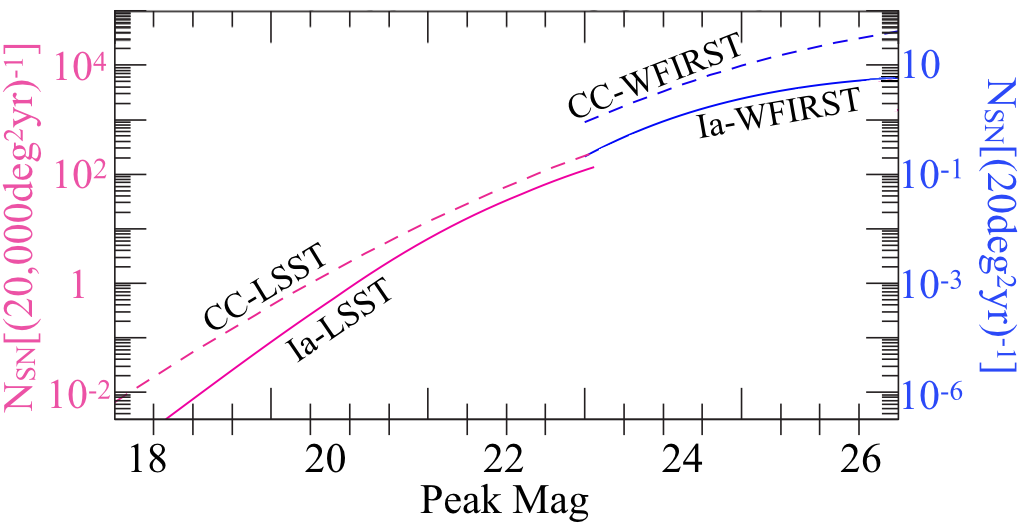
\includegraphics[width=.5\textwidth]{FIG/wfirst_lsst2}
\caption{
\noindent\fontsize{10}{14}\selectfont
Expected numbers of lensed SN Ia and Core Collapse SN after one year
of $20,000deg^2$ LSST (Pink, $i_{peak,lim})$ and $20deg^2$ WFIRST
(Blue, $H_{peak,lim})$ surveys. With this huge volume of lensed CC and
Ia SN observations expected in the next decade, the open-source SNTD
package will be widely used and essential for analyzing this large
WFIRST/LSST SN sample (adapted from Oguri $\&$ Marshall
2010 \nolink{\cite{Oguri:2010a}}).}
\end{wrapfigure}
\noindent\underline{\textit{Intellectual Merit}} : After completing SNTD, I
will use the software to make more precise time delay measurements for
the two currently documented multiply-imaged SN, and any others
discovered in the interim. Accurate measurements of the lensing
magnification and time delays for strongly lensed CC SN Refsdal can be
used to test models for the dark matter distribution in the lensing
object \nolink{\cite{Rodney:2015a,Rodney:2016}} or as a probe to test
cosmological models \cite{Suyu:2014}. For a multiply-imaged Type Ia
SN such as iPTF16geu, more accurate measurements will provide both an
important milestone in breaking degeneracies in the lens model and a
measurement of the Hubble constant $H_0$ that is completely
independent of the local distance
ladder \nolink{\cite{Kolatt:1998,Oguri:2003b}}. The methodology and software I
develop will be \textbf{be widely used by future SN surveys} for
analyzing multiply-imaged SN and tightening the constraints found in
the course of this work.

Over the next 2 years, I will measure the rates and properties for a
sample of high-z and lensed SN discovered with
the Hubble Space Telescope. This sample will draw from a series of HST programs (CLASH, \href{https://frontierfields.org}{FrontierSN}, \href{https://relics.stsci.edu/}{RELICS}, and the new \href{http://buffalo.ipac.caltech.edu/}{BUFFALO} survey) that have targeted massive galaxy clusters. I am currently collaborating with the team of
Dr. Rogier Windhorst on the JWST Guaranteed Time Observations (GTO)
program 1176. Beginning in 2019, this program will apply 110 hours of
cadenced imaging on massive galaxy clusters as well as a deep field at
the North Ecliptic Pole.  The GTO should deliver over 300 SN
detections for $z<5$, including a significant portion above the
current detection limit of $z\simeq2$, as well as a chance for
observations of Type Ia and Pair Instability (PI) SNe at $z>5$ (Figure
2). In addition to spurring return observations with HST and JWST,
this new sample of high-z SNe alone will enable tests of star
formation rates (SFR), the stellar initial mass function (IMF), SN
progenitor pathways, and explosion models for SNe in the early
Universe.
\begin{wrapfigure}{r}{.5\textwidth}
\centering
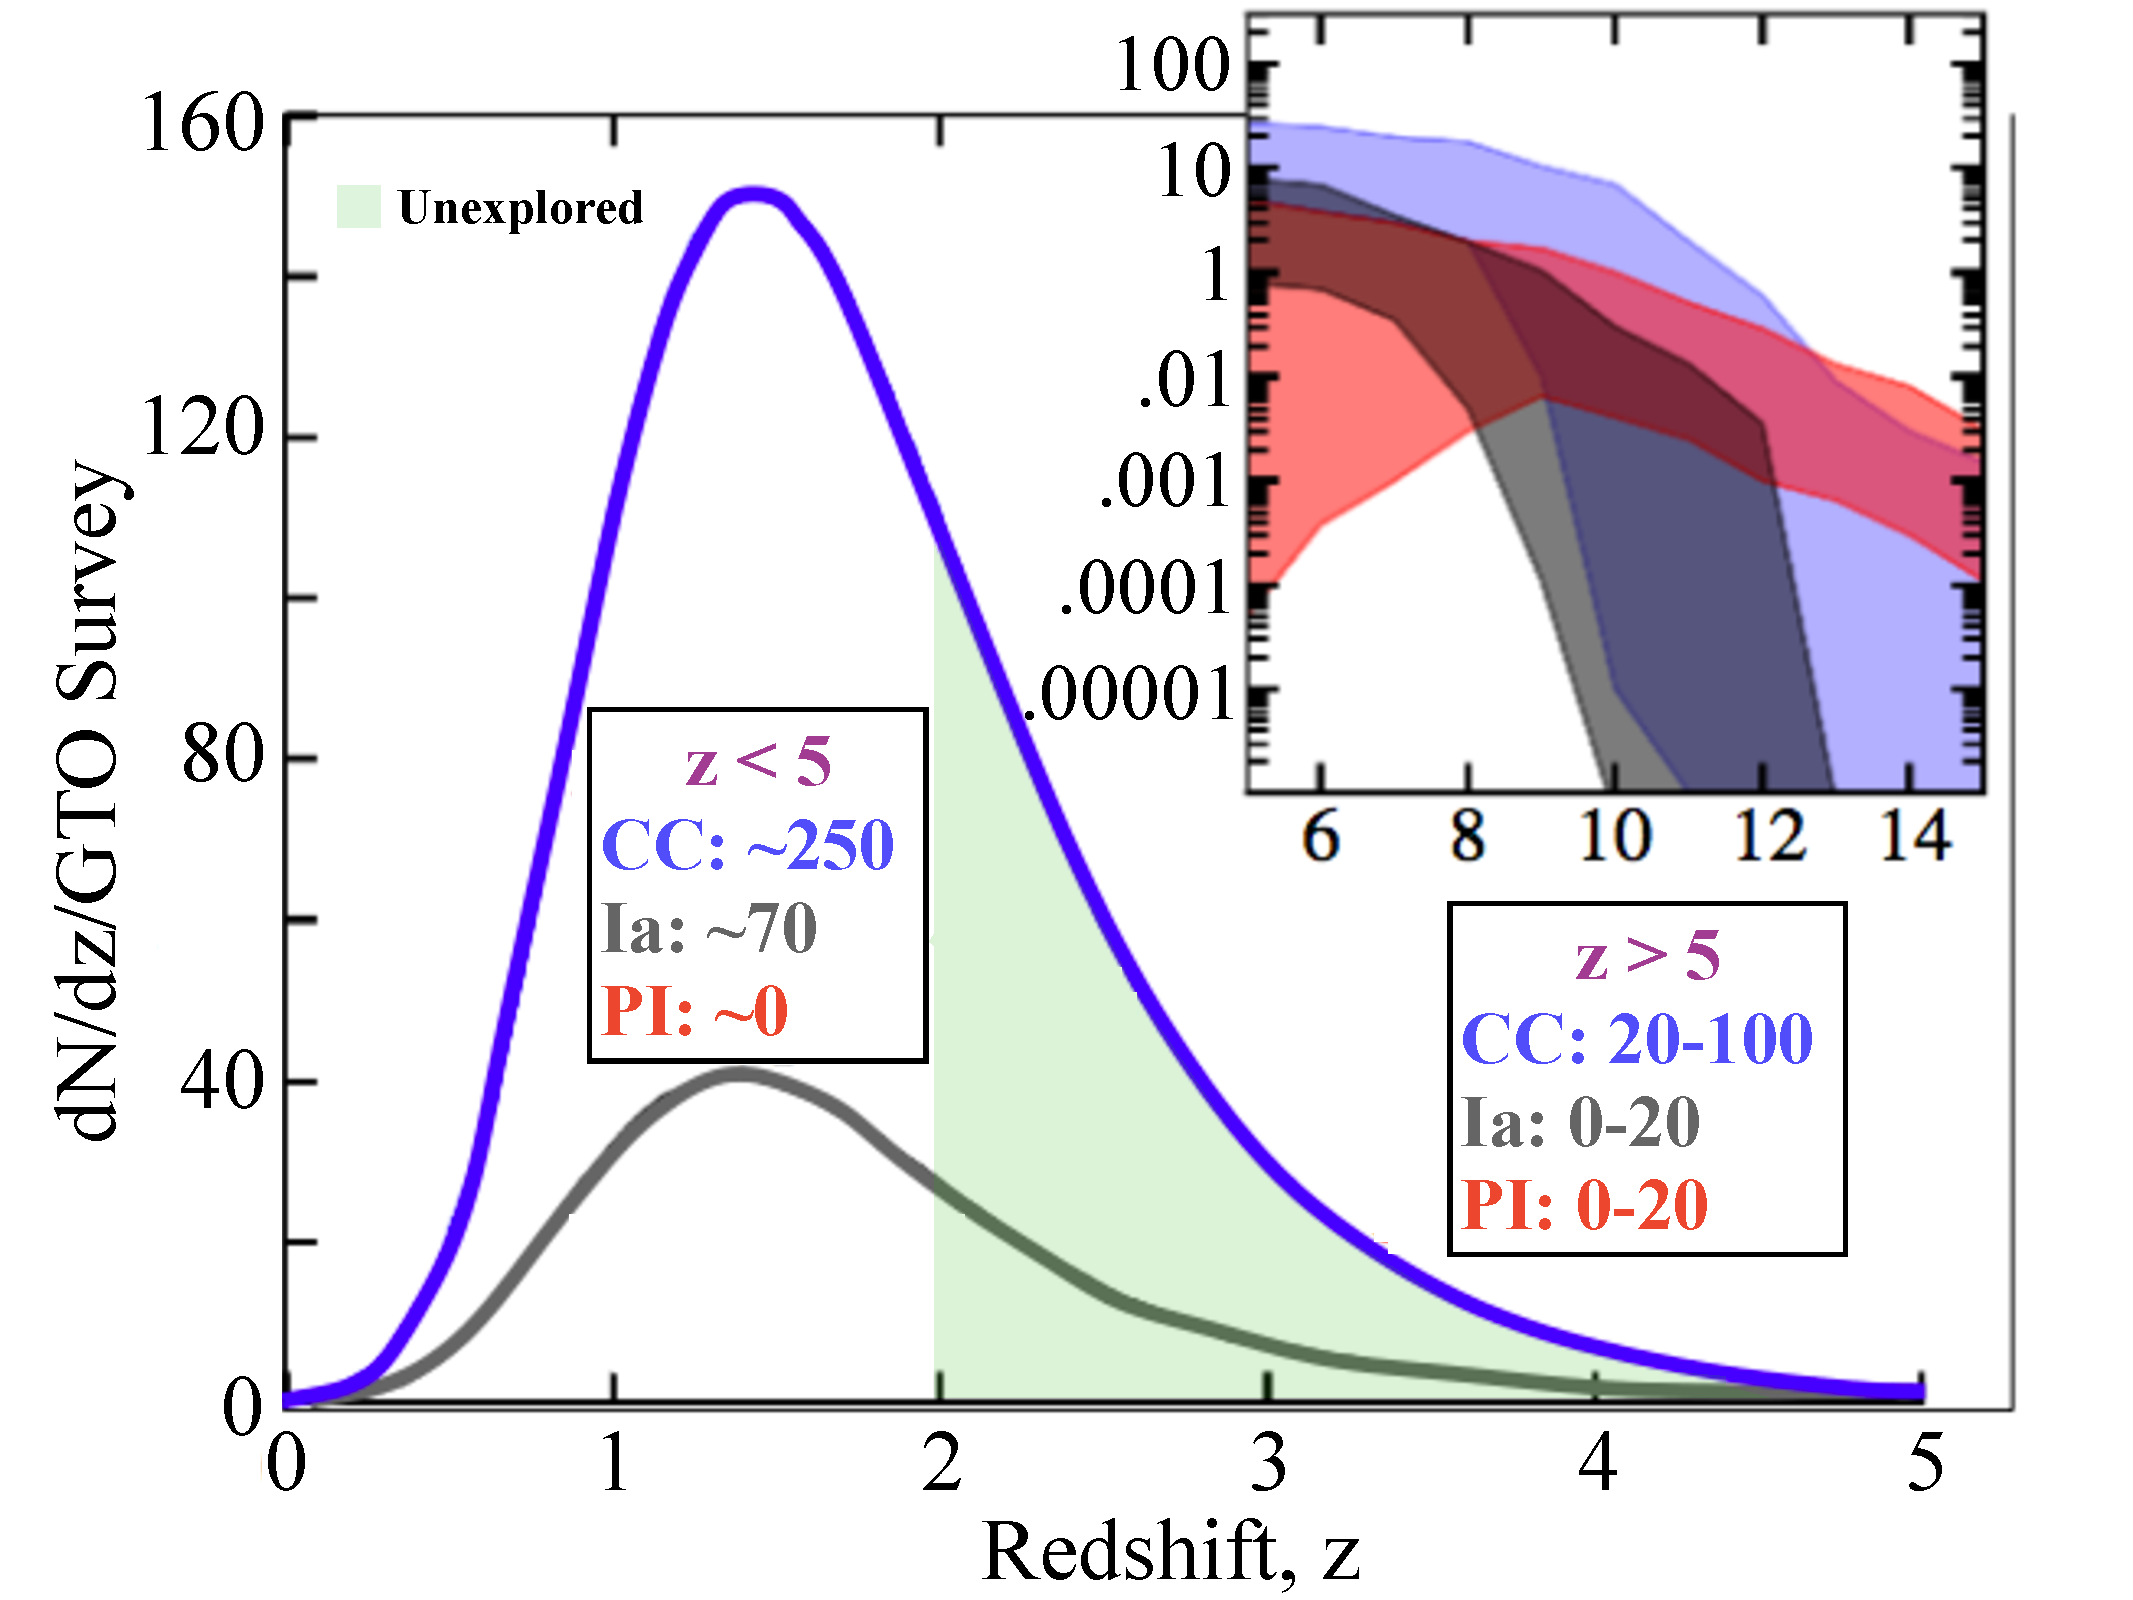
\includegraphics[height=.4\textwidth]{FIG/jwst_rates3}
%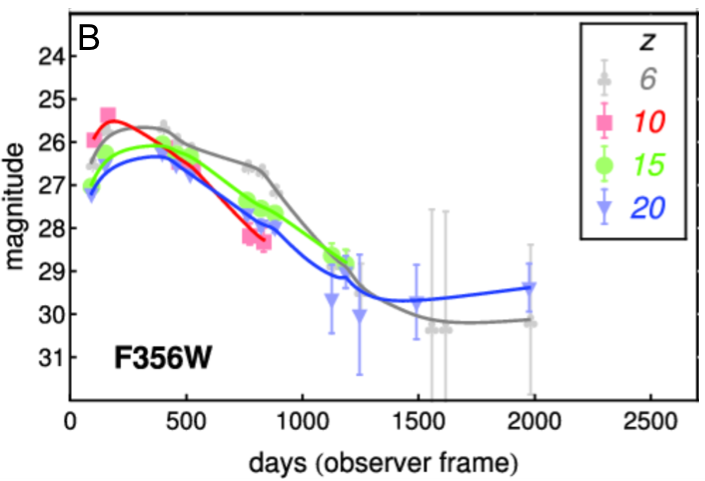
\includegraphics[height=.3\textwidth]{FIG/jwst_sim}
\caption{
\noindent\fontsize{10}{14}\selectfont
Projected SN yield from the JWST GTO 1176 program. We will
detect \textit{every} Type Ia SN that explodes in this field to z
$\lesssim5$ and 90$\%$ of all Core Collapse (CC) SNe to z $\simeq$
1.5, allowing the first high-z SN rate studies with an effectively
complete sample. The green region represents redshifts above the most
distant SN currently recorded, suggesting that observations from the
GTO will create a significant catalog of the most distant SNe yet
detected. The inset shows SN yield for $z>5$, where observations of early universe
Type Ia and PI SNe are possible.}
\end{wrapfigure}

\noindent\underline{\textit{Research Plan}}:
1)Complete the python software package SNTD and write a paper
presenting its capabilities and validation. 2) Perform reanalysis of
SN Refsdal and SN iPTF16geu using SNTD, writing a second paper
presenting the more precise time delay measurements, detailing the
methodology required for these analyses, and obtaining an initial
constraint on $H_0$ from iPTF16geu. 3)Form a sample of high-z and
lensed SNe from HST surveys and JWST GTO, and write a paper using this
sample to constrain the physical properties of SN progenitors in the
early universe.

\textbf{Evidence for the success of this work} will come from these \textbf{three publications}, as well as the vetting and
extensive use of the open-source SNTD package by the entire community
throughout future work with the next generation of space telescopes.

%Depending on the yield PISN

\noindent\underline{\textit{Broader Impacts}}:
I will use my previous STEM outreach experiences (see personal
statement) to \textbf{increase the participation of young students in
astronomy and other STEM fields from my neighborhood in Columbia, SC,
where 88$\%$ of the residents are underrepresented minorities in
STEM.}  My research is a terrific gateway into STEM because it is
naturally exciting and interesting: space telescopes, exploding stars,
and gravitational lensing are surefire topics to capture the attention
and imagination of a young learner. I have already created a plan with
the \textit{Lyon Street Community After School Program} that
will include taking the kids to our local University observatory, and
leading them through a series of astronomical
exercises over the course of the year. I will have each student choose
and carry out an astronomy project within our neighborhood, such as
monitoring sunspots to measure the rotation of the sun, and present
their results to the community. By teaching the students and engaging
their parents via the research projects and presentations, this outreach
program will \textbf{ encourage higher learning in STEM, and increase
public scientific literacy and public engagement with STEM}.

\noindent\fontsize{10}{14}\selectfont
[1]Kelly, P. L., et al. 2015, \href{http://arXiv.org/abs/1411.6009}{arXiv:1411.6009} [2]Goobar, A., et
al. 2016, \href{http://arXiv.org/abs/1611.00014v1}{arXiv:1611.00014v1} [3]Oguri, M., $\&$ Marshall, P. J. 2010, \href{http://arXiv.org/abs/arXiv:1001.2037v2}{arXiv:1001.2037v2} [4]Rodney, S. A., et al. 2015, \href{http://arXiv.org/abs/1505.06211}{arXiv:1505.06211}
[5]Rodney, S. A., et al. 2016, \href{http://arxiv.org/abs/1512.05734}{arxiv:1512.05734} [6]Suyu, S. H., et
al. 2014, \href{http://arXiv.org/abs/1306.4732}{arXiv:1306.4732} [7]Kolatt, T. S., $\&$ Bartelmann, M. 1998, \href{http://arXiv.org/abs/astro-ph/9708120}{arXiv:stro-ph/9708120} [8]Oguri, M., $\&$ Kawano, Y. 2003, \href{http://arXiv.org/abs/astro-ph/0211499}{arXiv:astro-ph/0211499}
\pagebreak








% Enter your analysis plan here.

%%%%%%%%%%%%%%%%%%%%%%%%%%%%%%%%%%%%%%%%%%%%%%%%%%%%%%%%%%%%%%%%%%%%%%%%%%%

%   3. MANAGEMENT PLAN
%       (see Section 9.7 of the Call for Proposals)
%
%  Provide a concise, but complete, management plan. This plan will be used
%  by the review panels to assess the likely scale of the proposed research
%  program. Proposers should include a schedule of the work required to
%  achieve the scientific goals of the program, a description of the roles of the
%  PI, CoIs, postdocs, and students who will perform the work, and a plan to
%  disseminate the results to the community.
%
%\budgetnarrative       % Do not delete this command. CALLS the Management Plan header in the Style File (IGNORE the command name of budgetnarrative
%\forceindent The first stage of this project is to produce an open-source software
package called Supernova Time Delays ({\tt SNTD}). The software is being
developed as an open-source project, and is already publicly
accessible on github (\url{https://github.com/jpierel14/sntd}).  {\tt SNTD}
relies on two other public software packages: Python Curve Shifting
({\tt PyCS}; \citealt{Tewes:2013a}) a tool developed for measurement of
quasar time delays, and the SN light curve analysis package {\tt sncosmo}
(\citep{Barbary:2014}). Our further development of {\tt SNTD} will proceed in three steps: 1)
Integrate SNCosmo and PyCS, producing a tool that can model
SN light curve data with the abilities present in either software
package; 2) Extend and optimize the lensing and microlensing algorithm
present in PyCS for SNe; 3) Simulate a large number of multiply-imaged
SN light curves using SNCosmo and test the ability of SNTD to
simultaneously determine SN and lensing parameters. This work will be
done primarily by graduate student PI Roberts-Pierel, under the
guidance of Co-I Rodney at USC.  We anticipate this will require 4-6
months of full time effort from the PI.

In parallel with the software development, we will improve the
photometry of the two multiply-imaged SNe (Refsdal and iPTF16geu) by
1) reprocessing the HST images using the most up-to-date AstroDrizzle
software; 2) developing new time-variable PSF models, based on stellar
sources within each image; and 3) deriving new photometric time
series, using multiple photometry packages to extract photometry from
both the template-subtracted difference images and directly from the
FLT files. Although SN Refsdal appeared in the Hubble Frontier Fields,
for this work it is necessary to reprocess the data separately from
the official HFF products, because we need to break it up into
separate epochs.  This component will require 4-6 months of part-time
work from the two Co-I's, supplemented by additional effort from the
grad student PI.

For the conclusion of this project, we will use the new SNTD package
to measure improved gravitational lensing parameters for SN Refsdal
and iPTF16geu.   We anticipate that the
SNTD package and the results of the new lensing analyses will be
separately published within 12 months of the start of this project.

%\bibliography{bibs/bibdesk}
\pagebreak
It has been over half a century since astrophysicist Sjur Refsdal
first developed the theory to enable the use of a gravitationally
lensed supernova (SN) resolved into multiple images as a cosmological
tool. The first multiply-imaged core-collapse (CC) and Type Ia SN,
Refsdal \nolink{\cite{Kelly:2015a}} and iPTF16geu \nolink{\cite{Goobar:2016}}
respectively, have been discovered in just the past 3 years. As the
light for each of the multiple images follows a different path through
the expanding universe and through the lensing potential, the SN
images appear delayed by hours (for galaxy-scale lenses) or years (for
cluster-scale lenses). These gravitational lenses are also important
tools for extending our SN sample into the early universe, beyond the
limit of current detections at $z\simeq2$. As PI on an ongoing HST
Archival Research Grant, \textbf{I am developing the first open-source
software for analysis of lensed SNe} (\textit{Supernova Time Delays}
[SNTD]).  This Python package will be essential for precise
measurements of lens properties and time delays from the hundreds of
multiply-imaged SN observations expected over the next decade (Figure
1), and despite its design for SNe will be valuable for lensed quasar
measurements as well. My research will have two major components:
1. Using SNTD and multiply-imaged SN as a cosmological
probe. 2. Observing and understanding the rates and physical
properties of very high-z SNe.

\begin{wrapfigure}{r}{.5\textwidth}
\centering
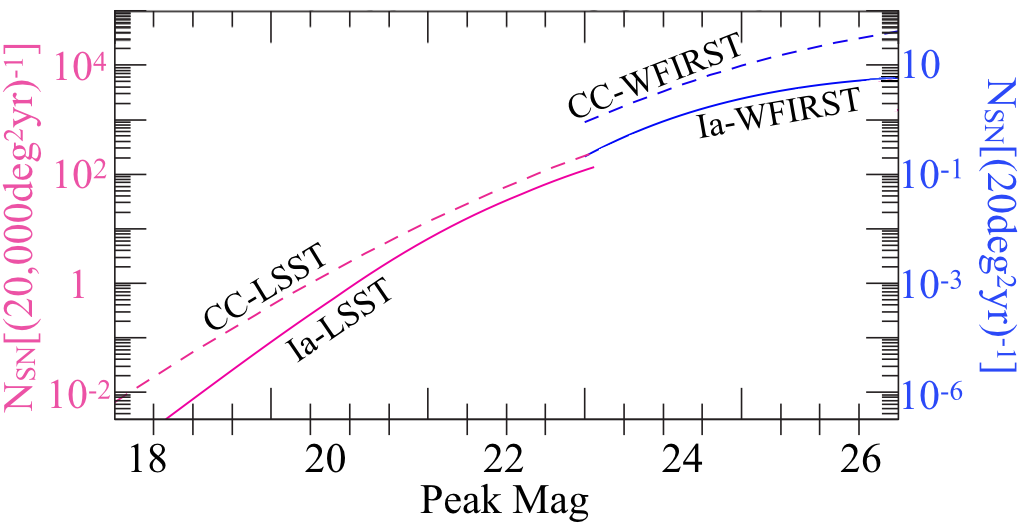
\includegraphics[width=.5\textwidth]{FIG/wfirst_lsst2}
\caption{
\noindent\fontsize{10}{14}\selectfont
Expected numbers of lensed SN Ia and Core Collapse SN after one year
of $20,000deg^2$ LSST (Pink, $i_{peak,lim})$ and $20deg^2$ WFIRST
(Blue, $H_{peak,lim})$ surveys. With this huge volume of lensed CC and
Ia SN observations expected in the next decade, the open-source SNTD
package will be widely used and essential for analyzing this large
WFIRST/LSST SN sample (adapted from Oguri $\&$ Marshall
2010 \nolink{\cite{Oguri:2010a}}).}
\end{wrapfigure}
\noindent\underline{\textit{Intellectual Merit}} : After completing SNTD, I
will use the software to make more precise time delay measurements for
the two currently documented multiply-imaged SN, and any others
discovered in the interim. Accurate measurements of the lensing
magnification and time delays for strongly lensed CC SN Refsdal can be
used to test models for the dark matter distribution in the lensing
object \nolink{\cite{Rodney:2015a,Rodney:2016}} or as a probe to test
cosmological models \cite{Suyu:2014}. For a multiply-imaged Type Ia
SN such as iPTF16geu, more accurate measurements will provide both an
important milestone in breaking degeneracies in the lens model and a
measurement of the Hubble constant $H_0$ that is completely
independent of the local distance
ladder \nolink{\cite{Kolatt:1998,Oguri:2003b}}. The methodology and software I
develop will be \textbf{be widely used by future SN surveys} for
analyzing multiply-imaged SN and tightening the constraints found in
the course of this work.

Over the next 2 years, I will measure the rates and properties for a
sample of high-z and lensed SN discovered with
the Hubble Space Telescope. This sample will draw from a series of HST programs (CLASH, \href{https://frontierfields.org}{FrontierSN}, \href{https://relics.stsci.edu/}{RELICS}, and the new \href{http://buffalo.ipac.caltech.edu/}{BUFFALO} survey) that have targeted massive galaxy clusters. I am currently collaborating with the team of
Dr. Rogier Windhorst on the JWST Guaranteed Time Observations (GTO)
program 1176. Beginning in 2019, this program will apply 110 hours of
cadenced imaging on massive galaxy clusters as well as a deep field at
the North Ecliptic Pole.  The GTO should deliver over 300 SN
detections for $z<5$, including a significant portion above the
current detection limit of $z\simeq2$, as well as a chance for
observations of Type Ia and Pair Instability (PI) SNe at $z>5$ (Figure
2). In addition to spurring return observations with HST and JWST,
this new sample of high-z SNe alone will enable tests of star
formation rates (SFR), the stellar initial mass function (IMF), SN
progenitor pathways, and explosion models for SNe in the early
Universe.
\begin{wrapfigure}{r}{.5\textwidth}
\centering
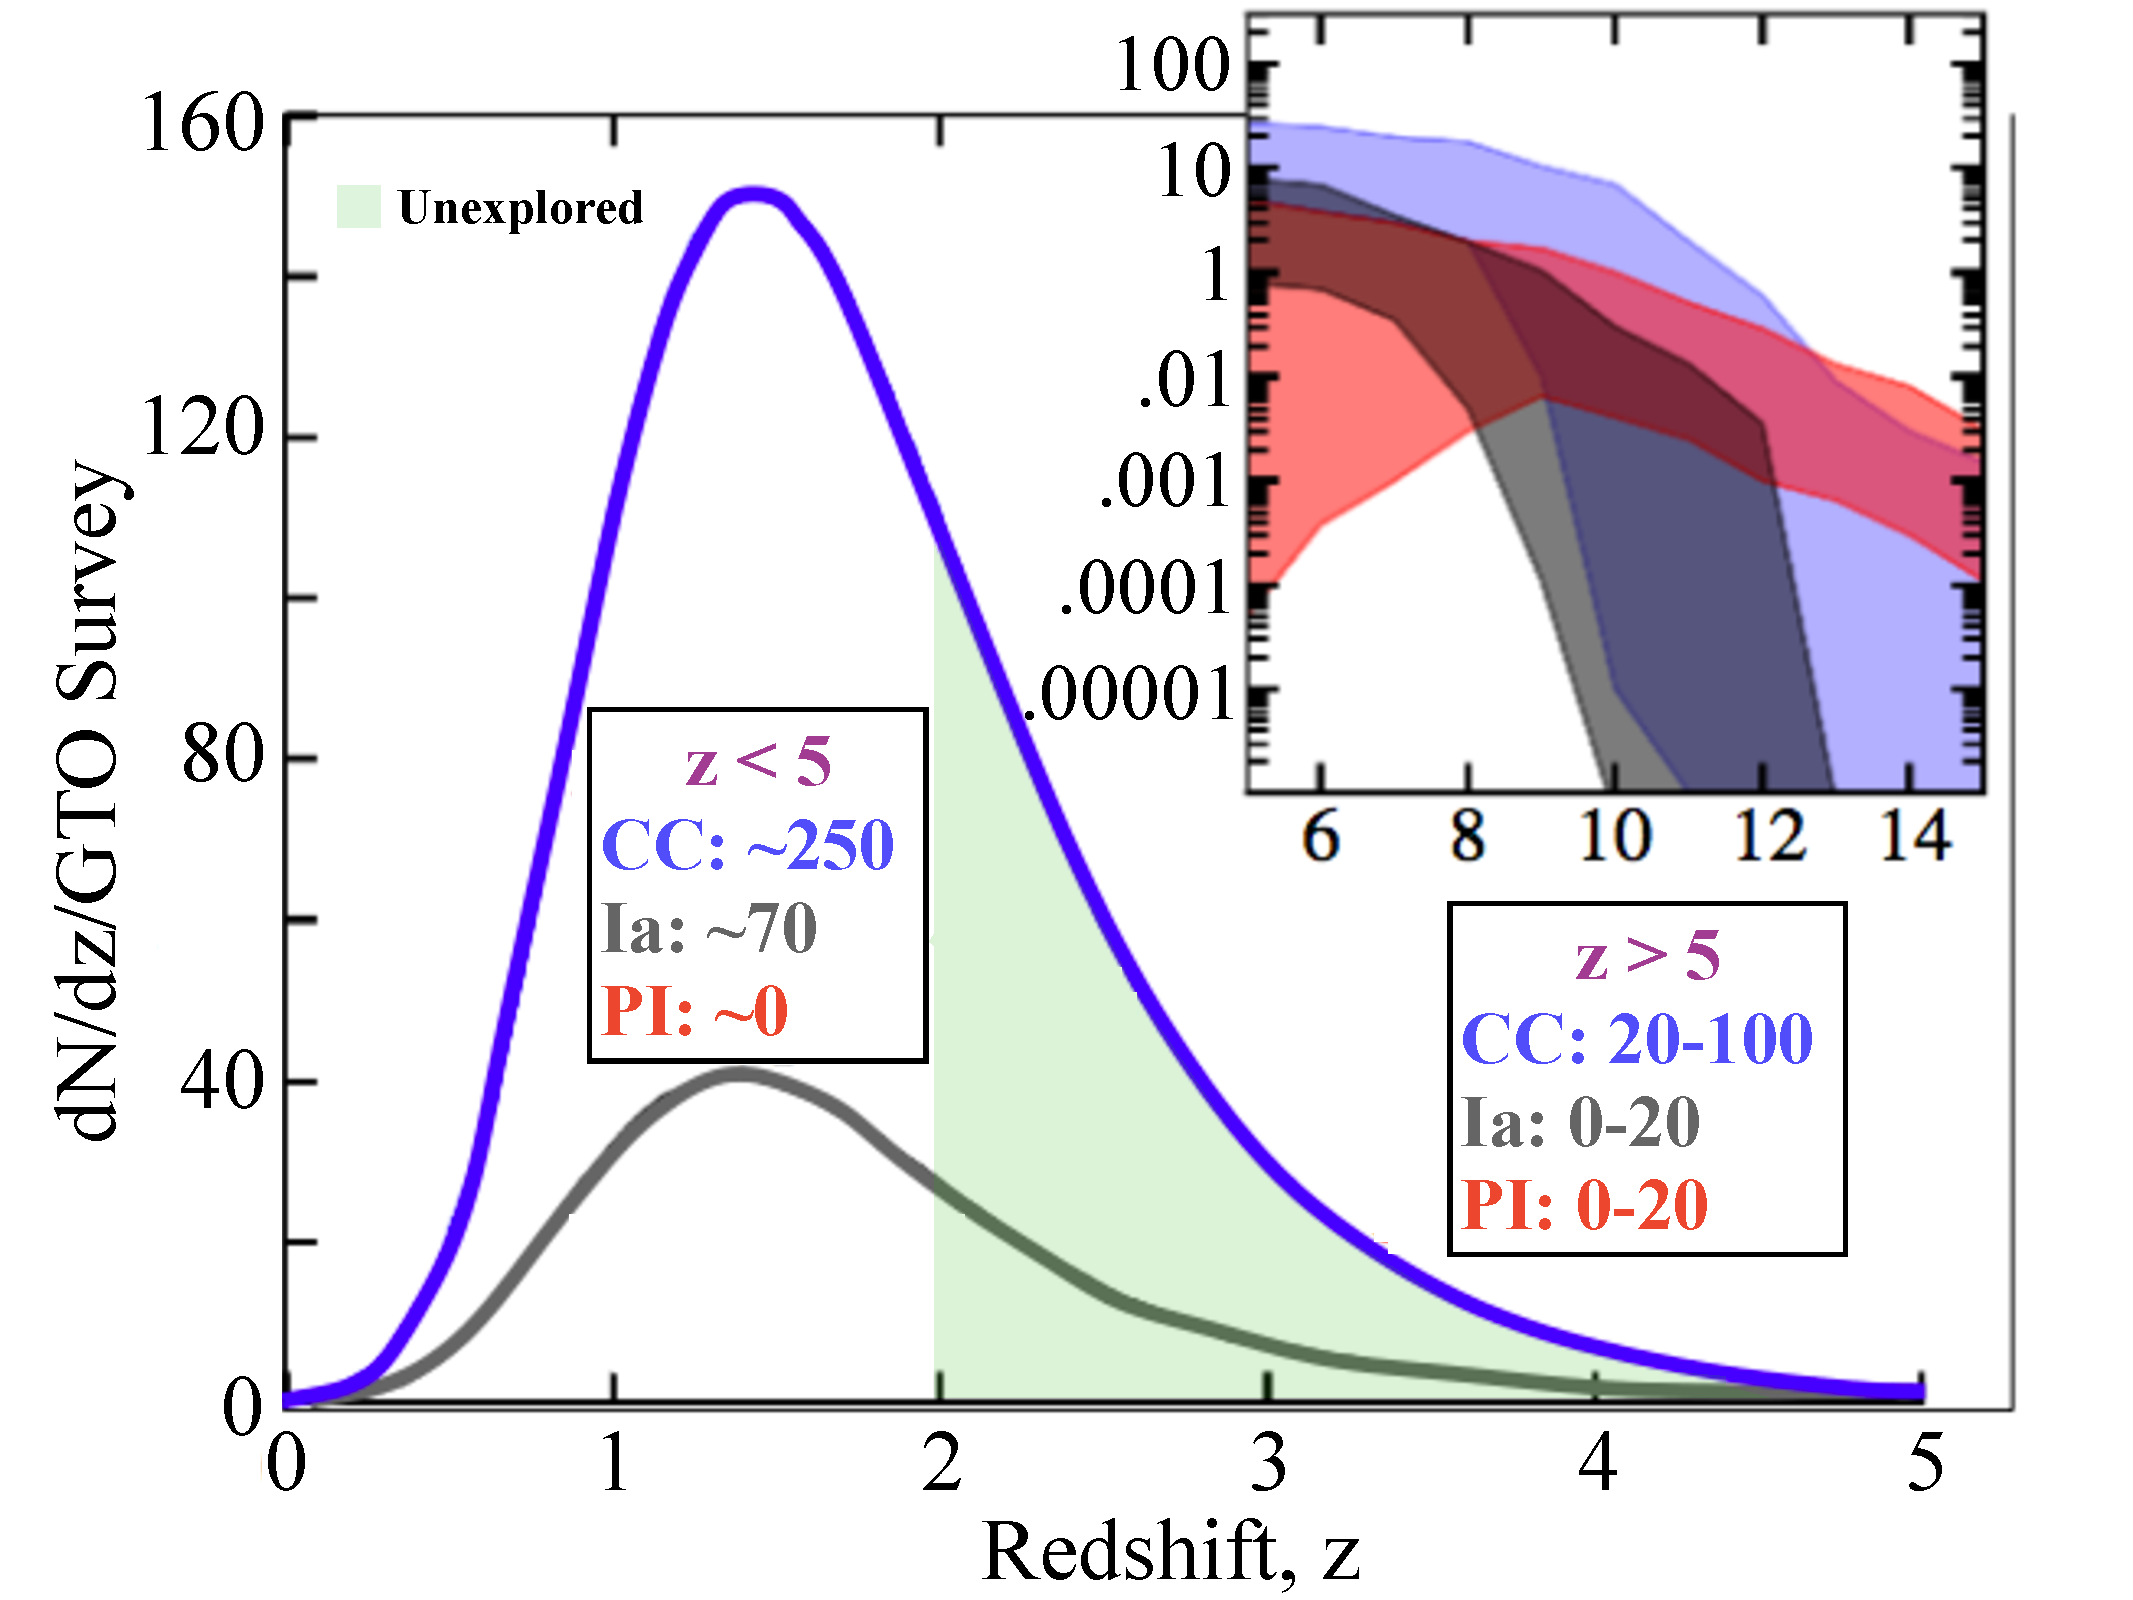
\includegraphics[height=.4\textwidth]{FIG/jwst_rates3}
%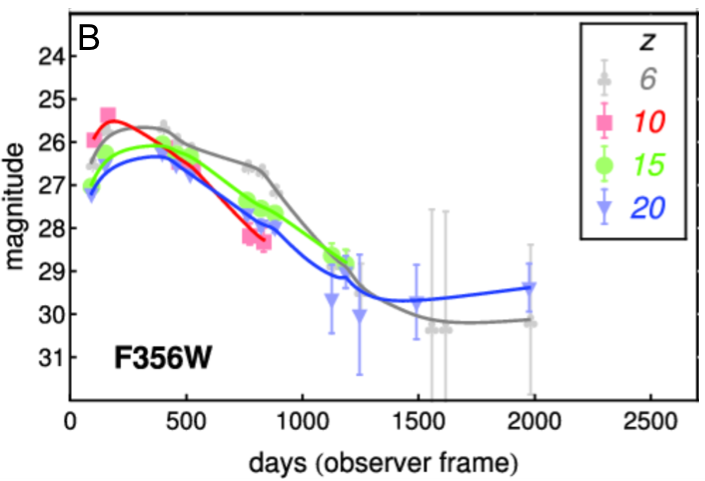
\includegraphics[height=.3\textwidth]{FIG/jwst_sim}
\caption{
\noindent\fontsize{10}{14}\selectfont
Projected SN yield from the JWST GTO 1176 program. We will
detect \textit{every} Type Ia SN that explodes in this field to z
$\lesssim5$ and 90$\%$ of all Core Collapse (CC) SNe to z $\simeq$
1.5, allowing the first high-z SN rate studies with an effectively
complete sample. The green region represents redshifts above the most
distant SN currently recorded, suggesting that observations from the
GTO will create a significant catalog of the most distant SNe yet
detected. The inset shows SN yield for $z>5$, where observations of early universe
Type Ia and PI SNe are possible.}
\end{wrapfigure}

\noindent\underline{\textit{Research Plan}}:
1)Complete the python software package SNTD and write a paper
presenting its capabilities and validation. 2) Perform reanalysis of
SN Refsdal and SN iPTF16geu using SNTD, writing a second paper
presenting the more precise time delay measurements, detailing the
methodology required for these analyses, and obtaining an initial
constraint on $H_0$ from iPTF16geu. 3)Form a sample of high-z and
lensed SNe from HST surveys and JWST GTO, and write a paper using this
sample to constrain the physical properties of SN progenitors in the
early universe.

\textbf{Evidence for the success of this work} will come from these \textbf{three publications}, as well as the vetting and
extensive use of the open-source SNTD package by the entire community
throughout future work with the next generation of space telescopes.

%Depending on the yield PISN

\noindent\underline{\textit{Broader Impacts}}:
I will use my previous STEM outreach experiences (see personal
statement) to \textbf{increase the participation of young students in
astronomy and other STEM fields from my neighborhood in Columbia, SC,
where 88$\%$ of the residents are underrepresented minorities in
STEM.}  My research is a terrific gateway into STEM because it is
naturally exciting and interesting: space telescopes, exploding stars,
and gravitational lensing are surefire topics to capture the attention
and imagination of a young learner. I have already created a plan with
the \textit{Lyon Street Community After School Program} that
will include taking the kids to our local University observatory, and
leading them through a series of astronomical
exercises over the course of the year. I will have each student choose
and carry out an astronomy project within our neighborhood, such as
monitoring sunspots to measure the rotation of the sun, and present
their results to the community. By teaching the students and engaging
their parents via the research projects and presentations, this outreach
program will \textbf{ encourage higher learning in STEM, and increase
public scientific literacy and public engagement with STEM}.

\noindent\fontsize{10}{14}\selectfont
[1]Kelly, P. L., et al. 2015, \href{http://arXiv.org/abs/1411.6009}{arXiv:1411.6009} [2]Goobar, A., et
al. 2016, \href{http://arXiv.org/abs/1611.00014v1}{arXiv:1611.00014v1} [3]Oguri, M., $\&$ Marshall, P. J. 2010, \href{http://arXiv.org/abs/arXiv:1001.2037v2}{arXiv:1001.2037v2} [4]Rodney, S. A., et al. 2015, \href{http://arXiv.org/abs/1505.06211}{arXiv:1505.06211}
[5]Rodney, S. A., et al. 2016, \href{http://arxiv.org/abs/1512.05734}{arxiv:1512.05734} [6]Suyu, S. H., et
al. 2014, \href{http://arXiv.org/abs/1306.4732}{arXiv:1306.4732} [7]Kolatt, T. S., $\&$ Bartelmann, M. 1998, \href{http://arXiv.org/abs/astro-ph/9708120}{arXiv:stro-ph/9708120} [8]Oguri, M., $\&$ Kawano, Y. 2003, \href{http://arXiv.org/abs/astro-ph/0211499}{arXiv:astro-ph/0211499}
\pagebreak








\bibliographystyle{apjbrief}
\pagebreak
\bibliography{bibs/bibdesk}

\end{document}          % End of proposal. Do not delete this line.
                        % Everything after this command is ignored.

